\chapter{Análisis de otras señales}
Utilizando señales (i)cuadradas, (ii)triangulares(simetría 50\%) y (iii)un tren de pulsos con $DC=33.3\%$
\begin{enumerate}
    \item Se analizó analíticamente el espectro de la señal
    \item Se simuló el espectro mediante MATLAB
    \item Se midió la señal con el analizador de espectros
    \item Se calculó el DC en función a la medición
\end{enumerate}

\section{Señal Cuadrada}
    \subsection{Análisis matemático}

    \begin{figure}[h]
        \begin{center}
            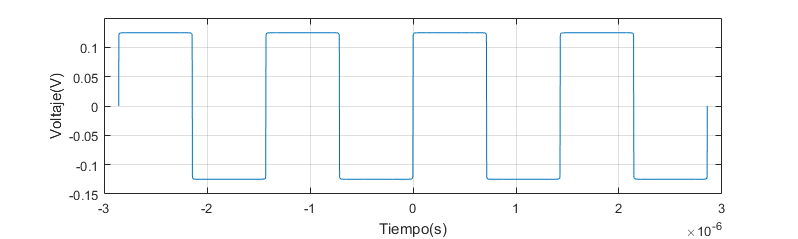
\includegraphics[width=\linewidth]{contenido/img/sig_sqr.png}
            \caption{Señal cuadrada con las características dadas}
            \label{fig:2,1,1}
        \end{center}
    \end{figure}

\section{Señal Triangular}

\section{Tren de Pulsos}